\documentclass[twoside]{book}

% Packages required by doxygen
\usepackage{fixltx2e}
\usepackage{calc}
\usepackage{doxygen}
\usepackage[export]{adjustbox} % also loads graphicx
\usepackage{graphicx}
\usepackage[utf8]{inputenc}
\usepackage{makeidx}
\usepackage{multicol}
\usepackage{multirow}
\PassOptionsToPackage{warn}{textcomp}
\usepackage{textcomp}
\usepackage[nointegrals]{wasysym}
\usepackage[table]{xcolor}

% Font selection
\usepackage[T1]{fontenc}
\usepackage[scaled=.90]{helvet}
\usepackage{courier}
\usepackage{amssymb}
\usepackage{sectsty}
\renewcommand{\familydefault}{\sfdefault}
\allsectionsfont{%
  \fontseries{bc}\selectfont%
  \color{darkgray}%
}
\renewcommand{\DoxyLabelFont}{%
  \fontseries{bc}\selectfont%
  \color{darkgray}%
}
\newcommand{\+}{\discretionary{\mbox{\scriptsize$\hookleftarrow$}}{}{}}

% Page & text layout
\usepackage{geometry}
\geometry{%
  a4paper,%
  top=2.5cm,%
  bottom=2.5cm,%
  left=2.5cm,%
  right=2.5cm%
}
\tolerance=750
\hfuzz=15pt
\hbadness=750
\setlength{\emergencystretch}{15pt}
\setlength{\parindent}{0cm}
\setlength{\parskip}{3ex plus 2ex minus 2ex}
\makeatletter
\renewcommand{\paragraph}{%
  \@startsection{paragraph}{4}{0ex}{-1.0ex}{1.0ex}{%
    \normalfont\normalsize\bfseries\SS@parafont%
  }%
}
\renewcommand{\subparagraph}{%
  \@startsection{subparagraph}{5}{0ex}{-1.0ex}{1.0ex}{%
    \normalfont\normalsize\bfseries\SS@subparafont%
  }%
}
\makeatother

% Headers & footers
\usepackage{fancyhdr}
\pagestyle{fancyplain}
\fancyhead[LE]{\fancyplain{}{\bfseries\thepage}}
\fancyhead[CE]{\fancyplain{}{}}
\fancyhead[RE]{\fancyplain{}{\bfseries\leftmark}}
\fancyhead[LO]{\fancyplain{}{\bfseries\rightmark}}
\fancyhead[CO]{\fancyplain{}{}}
\fancyhead[RO]{\fancyplain{}{\bfseries\thepage}}
\fancyfoot[LE]{\fancyplain{}{}}
\fancyfoot[CE]{\fancyplain{}{}}
\fancyfoot[RE]{\fancyplain{}{\bfseries\scriptsize Generated by Doxygen }}
\fancyfoot[LO]{\fancyplain{}{\bfseries\scriptsize Generated by Doxygen }}
\fancyfoot[CO]{\fancyplain{}{}}
\fancyfoot[RO]{\fancyplain{}{}}
\renewcommand{\footrulewidth}{0.4pt}
\renewcommand{\chaptermark}[1]{%
  \markboth{#1}{}%
}
\renewcommand{\sectionmark}[1]{%
  \markright{\thesection\ #1}%
}

% Indices & bibliography
\usepackage{natbib}
\usepackage[titles]{tocloft}
\setcounter{tocdepth}{3}
\setcounter{secnumdepth}{5}
\makeindex

% Hyperlinks (required, but should be loaded last)
\usepackage{ifpdf}
\ifpdf
  \usepackage[pdftex,pagebackref=true]{hyperref}
\else
  \usepackage[ps2pdf,pagebackref=true]{hyperref}
\fi
\hypersetup{%
  colorlinks=true,%
  linkcolor=blue,%
  citecolor=blue,%
  unicode%
}

% Custom commands
\newcommand{\clearemptydoublepage}{%
  \newpage{\pagestyle{empty}\cleardoublepage}%
}

\usepackage{caption}
\captionsetup{labelsep=space,justification=centering,font={bf},singlelinecheck=off,skip=4pt,position=top}

%===== C O N T E N T S =====

\begin{document}

% Titlepage & ToC
\hypersetup{pageanchor=false,
             bookmarksnumbered=true,
             pdfencoding=unicode
            }
\pagenumbering{alph}
\begin{titlepage}
\vspace*{7cm}
\begin{center}%
{\Large Exp\+\_\+assignment3 }\\
\vspace*{1cm}
{\large Generated by Doxygen 1.8.13}\\
\end{center}
\end{titlepage}
\clearemptydoublepage
\pagenumbering{roman}
\tableofcontents
\clearemptydoublepage
\pagenumbering{arabic}
\hypersetup{pageanchor=true}

%--- Begin generated contents ---
\chapter{Hierarchical Index}
\section{Class Hierarchy}
This inheritance list is sorted roughly, but not completely, alphabetically\+:\begin{DoxyCompactList}
\item \contentsline{section}{camera\+\_\+processing.\+Ball}{\pageref{classcamera__processing_1_1Ball}}{}
\item \contentsline{section}{camera\+\_\+processing.\+image\+\_\+feature}{\pageref{classcamera__processing_1_1image__feature}}{}
\item \contentsline{section}{State\+\_\+\+Machine.\+Room}{\pageref{classState__Machine_1_1Room}}{}
\item State\begin{DoxyCompactList}
\item \contentsline{section}{State\+\_\+\+Machine.\+Find}{\pageref{classState__Machine_1_1Find}}{}
\item \contentsline{section}{State\+\_\+\+Machine.\+Find\+\_\+\+Track}{\pageref{classState__Machine_1_1Find__Track}}{}
\item \contentsline{section}{State\+\_\+\+Machine.\+Normal}{\pageref{classState__Machine_1_1Normal}}{}
\item \contentsline{section}{State\+\_\+\+Machine.\+Normal\+\_\+\+Track}{\pageref{classState__Machine_1_1Normal__Track}}{}
\item \contentsline{section}{State\+\_\+\+Machine.\+Play}{\pageref{classState__Machine_1_1Play}}{}
\item \contentsline{section}{State\+\_\+\+Machine.\+Sleep}{\pageref{classState__Machine_1_1Sleep}}{}
\end{DoxyCompactList}
\end{DoxyCompactList}

\chapter{Class Index}
\section{Class List}
Here are the classes, structs, unions and interfaces with brief descriptions\+:\begin{DoxyCompactList}
\item\contentsline{section}{\hyperlink{classcamera__processing_1_1Ball}{camera\+\_\+processing.\+Ball} \\*Class for imformations about balls }{\pageref{classcamera__processing_1_1Ball}}{}
\item\contentsline{section}{\hyperlink{classState__Machine_1_1Find}{State\+\_\+\+Machine.\+Find} \\*\hyperlink{classState__Machine_1_1Find}{Find} State }{\pageref{classState__Machine_1_1Find}}{}
\item\contentsline{section}{\hyperlink{classState__Machine_1_1Find__Track}{State\+\_\+\+Machine.\+Find\+\_\+\+Track} \\*\hyperlink{classState__Machine_1_1Find}{Find} Track state }{\pageref{classState__Machine_1_1Find__Track}}{}
\item\contentsline{section}{\hyperlink{classcamera__processing_1_1image__feature}{camera\+\_\+processing.\+image\+\_\+feature} \\*Class for detecting and processing images }{\pageref{classcamera__processing_1_1image__feature}}{}
\item\contentsline{section}{\hyperlink{classState__Machine_1_1Normal}{State\+\_\+\+Machine.\+Normal} \\*\hyperlink{classState__Machine_1_1Normal}{Normal} State }{\pageref{classState__Machine_1_1Normal}}{}
\item\contentsline{section}{\hyperlink{classState__Machine_1_1Normal__Track}{State\+\_\+\+Machine.\+Normal\+\_\+\+Track} \\*\hyperlink{classState__Machine_1_1Normal__Track}{Normal\+\_\+\+Track} state }{\pageref{classState__Machine_1_1Normal__Track}}{}
\item\contentsline{section}{\hyperlink{classState__Machine_1_1Play}{State\+\_\+\+Machine.\+Play} \\*\hyperlink{classState__Machine_1_1Play}{Play} State }{\pageref{classState__Machine_1_1Play}}{}
\item\contentsline{section}{\hyperlink{classState__Machine_1_1Room}{State\+\_\+\+Machine.\+Room} \\*Class for storing informations about rooms }{\pageref{classState__Machine_1_1Room}}{}
\item\contentsline{section}{\hyperlink{classState__Machine_1_1Sleep}{State\+\_\+\+Machine.\+Sleep} \\*\hyperlink{classState__Machine_1_1Sleep}{Sleep} State }{\pageref{classState__Machine_1_1Sleep}}{}
\end{DoxyCompactList}

\chapter{File Index}
\section{File List}
Here is a list of all documented files with brief descriptions\+:\begin{DoxyCompactList}
\item\contentsline{section}{/home/sara/catkin\+\_\+ws/src/exp\+\_\+assignment3/scripts/\hyperlink{camera__processing_8py}{camera\+\_\+processing.\+py} \\*This node accesses to the camera, handles the images, founding the balls and sends all the informations about them to the state machine node }{\pageref{camera__processing_8py}}{}
\item\contentsline{section}{/home/sara/catkin\+\_\+ws/src/exp\+\_\+assignment3/scripts/\hyperlink{Commander_8py}{Commander.\+py} \\*This node chooses randomly the target and sends the command \char`\"{}\+Go\+To + target\char`\"{} to the state machine }{\pageref{Commander_8py}}{}
\item\contentsline{section}{/home/sara/catkin\+\_\+ws/src/exp\+\_\+assignment3/scripts/{\bfseries State\+\_\+\+Machine.\+py} }{\pageref{State__Machine_8py}}{}
\end{DoxyCompactList}

\chapter{Class Documentation}
\hypertarget{classcamera__processing_1_1Ball}{}\section{camera\+\_\+processing.\+Ball Class Reference}
\label{classcamera__processing_1_1Ball}\index{camera\+\_\+processing.\+Ball@{camera\+\_\+processing.\+Ball}}


class for imformations about balls  


\subsection*{Public Member Functions}
\begin{DoxyCompactItemize}
\item 
\mbox{\Hypertarget{classcamera__processing_1_1Ball_afe1bbcb95b732b87b8f33a8d39f7a1d5}\label{classcamera__processing_1_1Ball_afe1bbcb95b732b87b8f33a8d39f7a1d5}} 
def {\bfseries \+\_\+\+\_\+init\+\_\+\+\_\+} (self, color, lower, upper, radius, centerx, closeball, firstdetection)
\end{DoxyCompactItemize}
\subsection*{Public Attributes}
\begin{DoxyCompactItemize}
\item 
\mbox{\Hypertarget{classcamera__processing_1_1Ball_a6d7a8fbef513723d9c0069fa782fa4aa}\label{classcamera__processing_1_1Ball_a6d7a8fbef513723d9c0069fa782fa4aa}} 
{\bfseries color}
\item 
\mbox{\Hypertarget{classcamera__processing_1_1Ball_a1f02a5deead785f1a4d9b5940da8978d}\label{classcamera__processing_1_1Ball_a1f02a5deead785f1a4d9b5940da8978d}} 
{\bfseries lower}
\item 
\mbox{\Hypertarget{classcamera__processing_1_1Ball_a12abc5e4a2e9f6be6a6f72f5d8a968ec}\label{classcamera__processing_1_1Ball_a12abc5e4a2e9f6be6a6f72f5d8a968ec}} 
{\bfseries upper}
\item 
\mbox{\Hypertarget{classcamera__processing_1_1Ball_a90b066175e488951bbc95a363cf36526}\label{classcamera__processing_1_1Ball_a90b066175e488951bbc95a363cf36526}} 
{\bfseries detected}
\item 
\mbox{\Hypertarget{classcamera__processing_1_1Ball_a1464615c2d2082097be0d228862cebd0}\label{classcamera__processing_1_1Ball_a1464615c2d2082097be0d228862cebd0}} 
{\bfseries radius}
\item 
\mbox{\Hypertarget{classcamera__processing_1_1Ball_a4dfb4d242442048fe3499829abd246ad}\label{classcamera__processing_1_1Ball_a4dfb4d242442048fe3499829abd246ad}} 
{\bfseries centerx}
\item 
\mbox{\Hypertarget{classcamera__processing_1_1Ball_aa319ef3e0644868ca3f4dc345827f15f}\label{classcamera__processing_1_1Ball_aa319ef3e0644868ca3f4dc345827f15f}} 
{\bfseries closeball}
\item 
\mbox{\Hypertarget{classcamera__processing_1_1Ball_ac9673a422f961edc28b50132723bef58}\label{classcamera__processing_1_1Ball_ac9673a422f961edc28b50132723bef58}} 
{\bfseries firstdetection}
\end{DoxyCompactItemize}


\subsection{Detailed Description}
class for imformations about balls 

Definition at line 43 of file camera\+\_\+processing.\+py.



The documentation for this class was generated from the following file\+:\begin{DoxyCompactItemize}
\item 
/home/sara/catkin\+\_\+ws/src/exp\+\_\+assignment3/scripts/\hyperlink{camera__processing_8py}{camera\+\_\+processing.\+py}\end{DoxyCompactItemize}

\hypertarget{classState__Machine_1_1Find}{}\section{State\+\_\+\+Machine.\+Find Class Reference}
\label{classState__Machine_1_1Find}\index{State\+\_\+\+Machine.\+Find@{State\+\_\+\+Machine.\+Find}}


\hyperlink{classState__Machine_1_1Find}{Find} State.  




Inheritance diagram for State\+\_\+\+Machine.\+Find\+:
\nopagebreak
\begin{figure}[H]
\begin{center}
\leavevmode
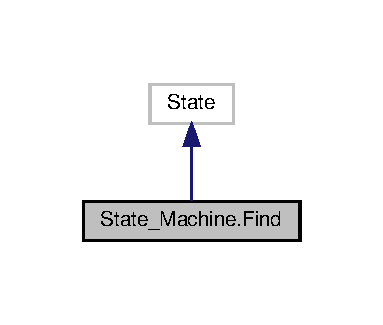
\includegraphics[width=184pt]{classState__Machine_1_1Find__inherit__graph}
\end{center}
\end{figure}


Collaboration diagram for State\+\_\+\+Machine.\+Find\+:
\nopagebreak
\begin{figure}[H]
\begin{center}
\leavevmode
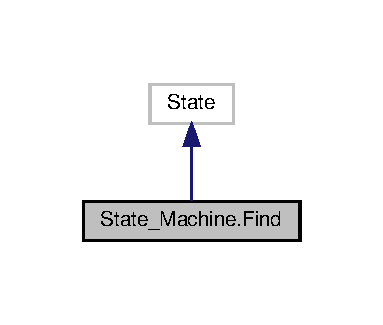
\includegraphics[width=184pt]{classState__Machine_1_1Find__coll__graph}
\end{center}
\end{figure}
\subsection*{Public Member Functions}
\begin{DoxyCompactItemize}
\item 
\mbox{\Hypertarget{classState__Machine_1_1Find_adacf0aacee7f880be6d8611f3692f258}\label{classState__Machine_1_1Find_adacf0aacee7f880be6d8611f3692f258}} 
def \hyperlink{classState__Machine_1_1Find_adacf0aacee7f880be6d8611f3692f258}{\+\_\+\+\_\+init\+\_\+\+\_\+} (self)
\begin{DoxyCompactList}\small\item\em inizialization \end{DoxyCompactList}\item 
\mbox{\Hypertarget{classState__Machine_1_1Find_a492e549177cf32a2aa5e715bfd66db53}\label{classState__Machine_1_1Find_a492e549177cf32a2aa5e715bfd66db53}} 
def \hyperlink{classState__Machine_1_1Find_a492e549177cf32a2aa5e715bfd66db53}{execute} (self, userdata)
\begin{DoxyCompactList}\small\item\em execution \end{DoxyCompactList}\end{DoxyCompactItemize}


\subsection{Detailed Description}
\hyperlink{classState__Machine_1_1Find}{Find} State. 

Definition at line 334 of file State\+\_\+\+Machine.\+py.



The documentation for this class was generated from the following file\+:\begin{DoxyCompactItemize}
\item 
/home/sara/catkin\+\_\+ws/src/exp\+\_\+assignment3/scripts/State\+\_\+\+Machine.\+py\end{DoxyCompactItemize}

\hypertarget{classState__Machine_1_1Find__Track}{}\section{State\+\_\+\+Machine.\+Find\+\_\+\+Track Class Reference}
\label{classState__Machine_1_1Find__Track}\index{State\+\_\+\+Machine.\+Find\+\_\+\+Track@{State\+\_\+\+Machine.\+Find\+\_\+\+Track}}


\hyperlink{classState__Machine_1_1Find}{Find} Track state.  




Inheritance diagram for State\+\_\+\+Machine.\+Find\+\_\+\+Track\+:
\nopagebreak
\begin{figure}[H]
\begin{center}
\leavevmode
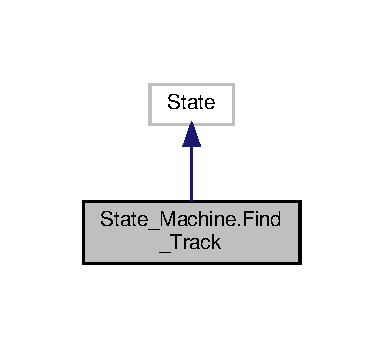
\includegraphics[width=184pt]{classState__Machine_1_1Find__Track__inherit__graph}
\end{center}
\end{figure}


Collaboration diagram for State\+\_\+\+Machine.\+Find\+\_\+\+Track\+:
\nopagebreak
\begin{figure}[H]
\begin{center}
\leavevmode
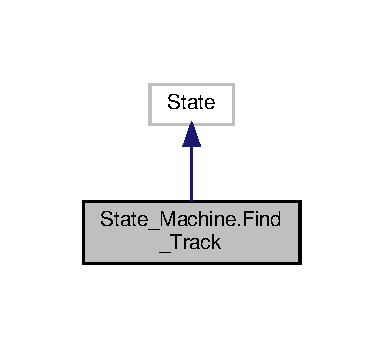
\includegraphics[width=184pt]{classState__Machine_1_1Find__Track__coll__graph}
\end{center}
\end{figure}
\subsection*{Public Member Functions}
\begin{DoxyCompactItemize}
\item 
\mbox{\Hypertarget{classState__Machine_1_1Find__Track_abfa42aea92e882a9a1011290337e412e}\label{classState__Machine_1_1Find__Track_abfa42aea92e882a9a1011290337e412e}} 
def \hyperlink{classState__Machine_1_1Find__Track_abfa42aea92e882a9a1011290337e412e}{\+\_\+\+\_\+init\+\_\+\+\_\+} (self)
\begin{DoxyCompactList}\small\item\em inizialization \end{DoxyCompactList}\item 
\mbox{\Hypertarget{classState__Machine_1_1Find__Track_a3c72cc1a7b85cf64567464d119641e5e}\label{classState__Machine_1_1Find__Track_a3c72cc1a7b85cf64567464d119641e5e}} 
def \hyperlink{classState__Machine_1_1Find__Track_a3c72cc1a7b85cf64567464d119641e5e}{execute} (self, userdata)
\begin{DoxyCompactList}\small\item\em execution \end{DoxyCompactList}\end{DoxyCompactItemize}


\subsection{Detailed Description}
\hyperlink{classState__Machine_1_1Find}{Find} Track state. 

Definition at line 368 of file State\+\_\+\+Machine.\+py.



The documentation for this class was generated from the following file\+:\begin{DoxyCompactItemize}
\item 
/home/sara/catkin\+\_\+ws/src/exp\+\_\+assignment3/scripts/State\+\_\+\+Machine.\+py\end{DoxyCompactItemize}

\hypertarget{classcamera__processing_1_1image__feature}{}\section{camera\+\_\+processing.\+image\+\_\+feature Class Reference}
\label{classcamera__processing_1_1image__feature}\index{camera\+\_\+processing.\+image\+\_\+feature@{camera\+\_\+processing.\+image\+\_\+feature}}


class for detecting and processing images  


\subsection*{Public Member Functions}
\begin{DoxyCompactItemize}
\item 
\mbox{\Hypertarget{classcamera__processing_1_1image__feature_af2c2bb646b34e9c602288a905d95630e}\label{classcamera__processing_1_1image__feature_af2c2bb646b34e9c602288a905d95630e}} 
def \hyperlink{classcamera__processing_1_1image__feature_af2c2bb646b34e9c602288a905d95630e}{\+\_\+\+\_\+init\+\_\+\+\_\+} (self)
\begin{DoxyCompactList}\small\item\em initialization \end{DoxyCompactList}\item 
\mbox{\Hypertarget{classcamera__processing_1_1image__feature_a0233f350c8ea996ef21e40fbeb38e1a3}\label{classcamera__processing_1_1image__feature_a0233f350c8ea996ef21e40fbeb38e1a3}} 
def \hyperlink{classcamera__processing_1_1image__feature_a0233f350c8ea996ef21e40fbeb38e1a3}{Det\+\_\+\+Ball\+\_\+clbk} (self, ros\+\_\+data)
\begin{DoxyCompactList}\small\item\em Callback. \end{DoxyCompactList}\end{DoxyCompactItemize}
\subsection*{Public Attributes}
\begin{DoxyCompactItemize}
\item 
\mbox{\Hypertarget{classcamera__processing_1_1image__feature_af5cc15149afabca31c3a04ccae179447}\label{classcamera__processing_1_1image__feature_af5cc15149afabca31c3a04ccae179447}} 
{\bfseries image\+\_\+pub}
\item 
\mbox{\Hypertarget{classcamera__processing_1_1image__feature_a4442e0932deffd1ed79922999ee5ace4}\label{classcamera__processing_1_1image__feature_a4442e0932deffd1ed79922999ee5ace4}} 
{\bfseries infos\+Ball\+\_\+pub}
\item 
\mbox{\Hypertarget{classcamera__processing_1_1image__feature_ae9134bd9aff3eaba9863e24da2667d21}\label{classcamera__processing_1_1image__feature_ae9134bd9aff3eaba9863e24da2667d21}} 
{\bfseries subscriber}
\end{DoxyCompactItemize}


\subsection{Detailed Description}
class for detecting and processing images 

Definition at line 63 of file camera\+\_\+processing.\+py.



The documentation for this class was generated from the following file\+:\begin{DoxyCompactItemize}
\item 
/home/sara/catkin\+\_\+ws/src/exp\+\_\+assignment3/scripts/\hyperlink{camera__processing_8py}{camera\+\_\+processing.\+py}\end{DoxyCompactItemize}

\hypertarget{classState__Machine_1_1Normal}{}\section{State\+\_\+\+Machine.\+Normal Class Reference}
\label{classState__Machine_1_1Normal}\index{State\+\_\+\+Machine.\+Normal@{State\+\_\+\+Machine.\+Normal}}


\hyperlink{classState__Machine_1_1Normal}{Normal} State.  




Inheritance diagram for State\+\_\+\+Machine.\+Normal\+:
\nopagebreak
\begin{figure}[H]
\begin{center}
\leavevmode
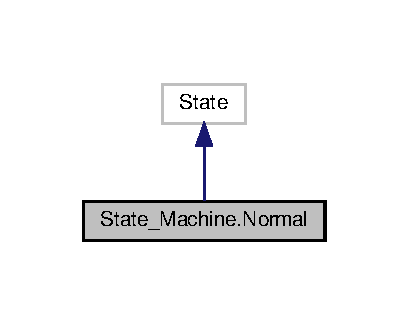
\includegraphics[width=196pt]{classState__Machine_1_1Normal__inherit__graph}
\end{center}
\end{figure}


Collaboration diagram for State\+\_\+\+Machine.\+Normal\+:
\nopagebreak
\begin{figure}[H]
\begin{center}
\leavevmode
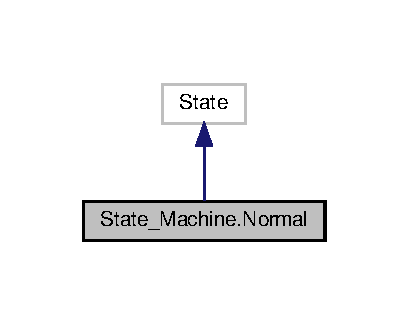
\includegraphics[width=196pt]{classState__Machine_1_1Normal__coll__graph}
\end{center}
\end{figure}
\subsection*{Public Member Functions}
\begin{DoxyCompactItemize}
\item 
\mbox{\Hypertarget{classState__Machine_1_1Normal_a517934b733d96f1a1bb530412f42da15}\label{classState__Machine_1_1Normal_a517934b733d96f1a1bb530412f42da15}} 
def \hyperlink{classState__Machine_1_1Normal_a517934b733d96f1a1bb530412f42da15}{\+\_\+\+\_\+init\+\_\+\+\_\+} (self)
\begin{DoxyCompactList}\small\item\em inizialization \end{DoxyCompactList}\item 
\mbox{\Hypertarget{classState__Machine_1_1Normal_aad25695eb358f21389fcf7122070dae4}\label{classState__Machine_1_1Normal_aad25695eb358f21389fcf7122070dae4}} 
def \hyperlink{classState__Machine_1_1Normal_aad25695eb358f21389fcf7122070dae4}{execute} (self, userdata)
\begin{DoxyCompactList}\small\item\em execution \end{DoxyCompactList}\end{DoxyCompactItemize}
\subsection*{Public Attributes}
\begin{DoxyCompactItemize}
\item 
\hyperlink{classState__Machine_1_1Normal_a390f2d9125adec1edb43339a27bd256e}{user\+Action}
\begin{DoxyCompactList}\small\item\em 3 outcomes defined \end{DoxyCompactList}\end{DoxyCompactItemize}


\subsection{Detailed Description}
\hyperlink{classState__Machine_1_1Normal}{Normal} State. 

Definition at line 181 of file State\+\_\+\+Machine.\+py.



\subsection{Member Data Documentation}
\mbox{\Hypertarget{classState__Machine_1_1Normal_a390f2d9125adec1edb43339a27bd256e}\label{classState__Machine_1_1Normal_a390f2d9125adec1edb43339a27bd256e}} 
\index{State\+\_\+\+Machine\+::\+Normal@{State\+\_\+\+Machine\+::\+Normal}!user\+Action@{user\+Action}}
\index{user\+Action@{user\+Action}!State\+\_\+\+Machine\+::\+Normal@{State\+\_\+\+Machine\+::\+Normal}}
\subsubsection{\texorpdfstring{user\+Action}{userAction}}
{\footnotesize\ttfamily State\+\_\+\+Machine.\+Normal.\+user\+Action}



3 outcomes defined 

look at the target

if play behavior is chosen

in loop

couter Random motion implementing a move\+\_\+base action with a random goal if camera detects a new ball which has not been detected before after 3 random goal achieved it can switch in sleep or play behavior (randomly choosen) call the function to randomly choose the next behavior

if the sleep behavoir is chosen 

Definition at line 187 of file State\+\_\+\+Machine.\+py.



The documentation for this class was generated from the following file\+:\begin{DoxyCompactItemize}
\item 
/home/sara/catkin\+\_\+ws/src/exp\+\_\+assignment3/scripts/State\+\_\+\+Machine.\+py\end{DoxyCompactItemize}

\hypertarget{classState__Machine_1_1Normal__Track}{}\section{State\+\_\+\+Machine.\+Normal\+\_\+\+Track Class Reference}
\label{classState__Machine_1_1Normal__Track}\index{State\+\_\+\+Machine.\+Normal\+\_\+\+Track@{State\+\_\+\+Machine.\+Normal\+\_\+\+Track}}


\hyperlink{classState__Machine_1_1Normal__Track}{Normal\+\_\+\+Track} state.  




Inheritance diagram for State\+\_\+\+Machine.\+Normal\+\_\+\+Track\+:
\nopagebreak
\begin{figure}[H]
\begin{center}
\leavevmode
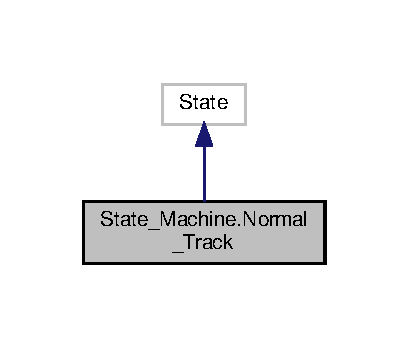
\includegraphics[width=196pt]{classState__Machine_1_1Normal__Track__inherit__graph}
\end{center}
\end{figure}


Collaboration diagram for State\+\_\+\+Machine.\+Normal\+\_\+\+Track\+:
\nopagebreak
\begin{figure}[H]
\begin{center}
\leavevmode
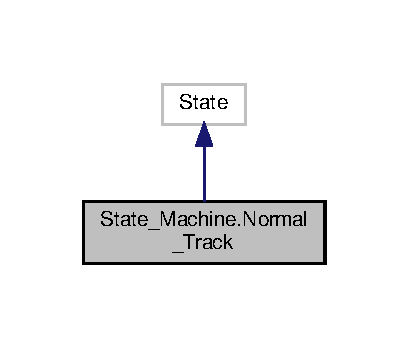
\includegraphics[width=196pt]{classState__Machine_1_1Normal__Track__coll__graph}
\end{center}
\end{figure}
\subsection*{Public Member Functions}
\begin{DoxyCompactItemize}
\item 
\mbox{\Hypertarget{classState__Machine_1_1Normal__Track_abe253cd840c44ccd24ad680b1092422c}\label{classState__Machine_1_1Normal__Track_abe253cd840c44ccd24ad680b1092422c}} 
def \hyperlink{classState__Machine_1_1Normal__Track_abe253cd840c44ccd24ad680b1092422c}{\+\_\+\+\_\+init\+\_\+\+\_\+} (self)
\begin{DoxyCompactList}\small\item\em inizialization \end{DoxyCompactList}\item 
\mbox{\Hypertarget{classState__Machine_1_1Normal__Track_a4878aa8a2963079bcab7fc838d498dc3}\label{classState__Machine_1_1Normal__Track_a4878aa8a2963079bcab7fc838d498dc3}} 
def \hyperlink{classState__Machine_1_1Normal__Track_a4878aa8a2963079bcab7fc838d498dc3}{execute} (self, userdata)
\begin{DoxyCompactList}\small\item\em execution \end{DoxyCompactList}\end{DoxyCompactItemize}


\subsection{Detailed Description}
\hyperlink{classState__Machine_1_1Normal__Track}{Normal\+\_\+\+Track} state. 

Definition at line 241 of file State\+\_\+\+Machine.\+py.



The documentation for this class was generated from the following file\+:\begin{DoxyCompactItemize}
\item 
/home/sara/catkin\+\_\+ws/src/exp\+\_\+assignment3/scripts/State\+\_\+\+Machine.\+py\end{DoxyCompactItemize}

\hypertarget{classState__Machine_1_1Play}{}\section{State\+\_\+\+Machine.\+Play Class Reference}
\label{classState__Machine_1_1Play}\index{State\+\_\+\+Machine.\+Play@{State\+\_\+\+Machine.\+Play}}


\hyperlink{classState__Machine_1_1Play}{Play} State.  




Inheritance diagram for State\+\_\+\+Machine.\+Play\+:
\nopagebreak
\begin{figure}[H]
\begin{center}
\leavevmode
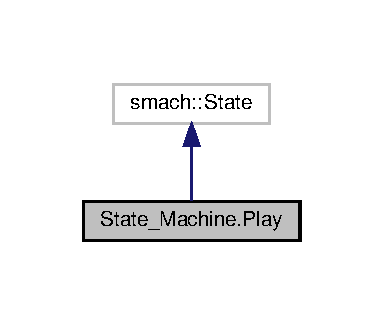
\includegraphics[width=184pt]{classState__Machine_1_1Play__inherit__graph}
\end{center}
\end{figure}


Collaboration diagram for State\+\_\+\+Machine.\+Play\+:
\nopagebreak
\begin{figure}[H]
\begin{center}
\leavevmode
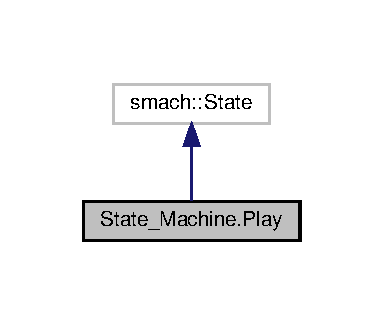
\includegraphics[width=184pt]{classState__Machine_1_1Play__coll__graph}
\end{center}
\end{figure}
\subsection*{Public Member Functions}
\begin{DoxyCompactItemize}
\item 
\mbox{\Hypertarget{classState__Machine_1_1Play_a1f62c75a5c32f90ff7ee5aecd4111a0f}\label{classState__Machine_1_1Play_a1f62c75a5c32f90ff7ee5aecd4111a0f}} 
def \hyperlink{classState__Machine_1_1Play_a1f62c75a5c32f90ff7ee5aecd4111a0f}{\+\_\+\+\_\+init\+\_\+\+\_\+} (self)
\begin{DoxyCompactList}\small\item\em inizialization \end{DoxyCompactList}\item 
\mbox{\Hypertarget{classState__Machine_1_1Play_a8b230b99cd16a8349e08f2c110b66482}\label{classState__Machine_1_1Play_a8b230b99cd16a8349e08f2c110b66482}} 
def \hyperlink{classState__Machine_1_1Play_a8b230b99cd16a8349e08f2c110b66482}{execute} (self, userdata)
\begin{DoxyCompactList}\small\item\em execution \end{DoxyCompactList}\end{DoxyCompactItemize}


\subsection{Detailed Description}
\hyperlink{classState__Machine_1_1Play}{Play} State. 

Definition at line 300 of file State\+\_\+\+Machine.\+py.



The documentation for this class was generated from the following file\+:\begin{DoxyCompactItemize}
\item 
/home/sara/catkin\+\_\+ws/src/exp\+\_\+assignment3/scripts/State\+\_\+\+Machine.\+py\end{DoxyCompactItemize}

\hypertarget{classState__Machine_1_1Room}{}\section{State\+\_\+\+Machine.\+Room Class Reference}
\label{classState__Machine_1_1Room}\index{State\+\_\+\+Machine.\+Room@{State\+\_\+\+Machine.\+Room}}


class for storing informations about rooms  


\subsection*{Public Member Functions}
\begin{DoxyCompactItemize}
\item 
\mbox{\Hypertarget{classState__Machine_1_1Room_a65464d35fe951e0f35c4b2a501737439}\label{classState__Machine_1_1Room_a65464d35fe951e0f35c4b2a501737439}} 
def {\bfseries \+\_\+\+\_\+init\+\_\+\+\_\+} (self, name, color, x, y)
\end{DoxyCompactItemize}
\subsection*{Public Attributes}
\begin{DoxyCompactItemize}
\item 
\mbox{\Hypertarget{classState__Machine_1_1Room_a3d30652341706ded27318643458d4da6}\label{classState__Machine_1_1Room_a3d30652341706ded27318643458d4da6}} 
{\bfseries name}
\item 
\mbox{\Hypertarget{classState__Machine_1_1Room_a9b4b6bb5ab572dbd3a86d2ce593fa9d7}\label{classState__Machine_1_1Room_a9b4b6bb5ab572dbd3a86d2ce593fa9d7}} 
{\bfseries color}
\item 
\mbox{\Hypertarget{classState__Machine_1_1Room_a27daffab86b6888691583c7ae21dd76f}\label{classState__Machine_1_1Room_a27daffab86b6888691583c7ae21dd76f}} 
{\bfseries x}
\item 
\mbox{\Hypertarget{classState__Machine_1_1Room_a05d9a05c6f4c72b6d0e6af24f6ce4fb4}\label{classState__Machine_1_1Room_a05d9a05c6f4c72b6d0e6af24f6ce4fb4}} 
{\bfseries y}
\end{DoxyCompactItemize}


\subsection{Detailed Description}
class for storing informations about rooms 

Definition at line 156 of file State\+\_\+\+Machine.\+py.



The documentation for this class was generated from the following file\+:\begin{DoxyCompactItemize}
\item 
/home/sara/catkin\+\_\+ws/src/exp\+\_\+assignment3/scripts/State\+\_\+\+Machine.\+py\end{DoxyCompactItemize}

\hypertarget{classState__Machine_1_1Sleep}{}\section{State\+\_\+\+Machine.\+Sleep Class Reference}
\label{classState__Machine_1_1Sleep}\index{State\+\_\+\+Machine.\+Sleep@{State\+\_\+\+Machine.\+Sleep}}


\hyperlink{classState__Machine_1_1Sleep}{Sleep} State.  




Inheritance diagram for State\+\_\+\+Machine.\+Sleep\+:
\nopagebreak
\begin{figure}[H]
\begin{center}
\leavevmode
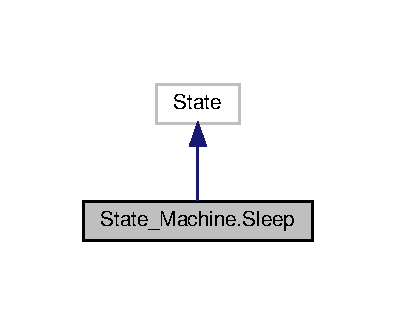
\includegraphics[width=190pt]{classState__Machine_1_1Sleep__inherit__graph}
\end{center}
\end{figure}


Collaboration diagram for State\+\_\+\+Machine.\+Sleep\+:
\nopagebreak
\begin{figure}[H]
\begin{center}
\leavevmode
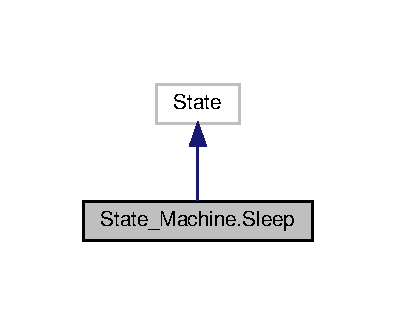
\includegraphics[width=190pt]{classState__Machine_1_1Sleep__coll__graph}
\end{center}
\end{figure}
\subsection*{Public Member Functions}
\begin{DoxyCompactItemize}
\item 
\mbox{\Hypertarget{classState__Machine_1_1Sleep_a80fe4b057086e30543d48b465fb46e66}\label{classState__Machine_1_1Sleep_a80fe4b057086e30543d48b465fb46e66}} 
def \hyperlink{classState__Machine_1_1Sleep_a80fe4b057086e30543d48b465fb46e66}{\+\_\+\+\_\+init\+\_\+\+\_\+} (self)
\begin{DoxyCompactList}\small\item\em inizialization \end{DoxyCompactList}\item 
\mbox{\Hypertarget{classState__Machine_1_1Sleep_a7ab46952ff37e2c2a15e545df30149ff}\label{classState__Machine_1_1Sleep_a7ab46952ff37e2c2a15e545df30149ff}} 
def \hyperlink{classState__Machine_1_1Sleep_a7ab46952ff37e2c2a15e545df30149ff}{execute} (self, userdata)
\begin{DoxyCompactList}\small\item\em execution \end{DoxyCompactList}\end{DoxyCompactItemize}


\subsection{Detailed Description}
\hyperlink{classState__Machine_1_1Sleep}{Sleep} State. 

Definition at line 280 of file State\+\_\+\+Machine.\+py.



The documentation for this class was generated from the following file\+:\begin{DoxyCompactItemize}
\item 
/home/sara/catkin\+\_\+ws/src/exp\+\_\+assignment3/scripts/State\+\_\+\+Machine.\+py\end{DoxyCompactItemize}

\chapter{File Documentation}
\hypertarget{camera__processing_8py}{}\section{/home/sara/catkin\+\_\+ws/src/exp\+\_\+assignment3/scripts/camera\+\_\+processing.py File Reference}
\label{camera__processing_8py}\index{/home/sara/catkin\+\_\+ws/src/exp\+\_\+assignment3/scripts/camera\+\_\+processing.\+py@{/home/sara/catkin\+\_\+ws/src/exp\+\_\+assignment3/scripts/camera\+\_\+processing.\+py}}


This node accesses to the camera, handles the images, founding the balls and sends all the informations about them to the state machine node.  


\subsection*{Classes}
\begin{DoxyCompactItemize}
\item 
class \hyperlink{classcamera__processing_1_1Ball}{camera\+\_\+processing.\+Ball}
\begin{DoxyCompactList}\small\item\em class for imformations about balls \end{DoxyCompactList}\item 
class \hyperlink{classcamera__processing_1_1image__feature}{camera\+\_\+processing.\+image\+\_\+feature}
\begin{DoxyCompactList}\small\item\em class for detecting and processing images \end{DoxyCompactList}\end{DoxyCompactItemize}
\subsection*{Functions}
\begin{DoxyCompactItemize}
\item 
\mbox{\Hypertarget{camera__processing_8py_a477673f68990bf32238aa68ec3a7a884}\label{camera__processing_8py_a477673f68990bf32238aa68ec3a7a884}} 
def \hyperlink{camera__processing_8py_a477673f68990bf32238aa68ec3a7a884}{camera\+\_\+processing.\+main} ()
\begin{DoxyCompactList}\small\item\em main \end{DoxyCompactList}\end{DoxyCompactItemize}
\subsection*{Variables}
\begin{DoxyCompactItemize}
\item 
list \hyperlink{camera__processing_8py_ae75cec8f3976b4d7574755f9c0dcb80e}{camera\+\_\+processing.\+balls}
\begin{DoxyCompactList}\small\item\em initialization of balls \end{DoxyCompactList}\end{DoxyCompactItemize}


\subsection{Detailed Description}
This node accesses to the camera, handles the images, founding the balls and sends all the informations about them to the state machine node. 



\subsection{Variable Documentation}
\mbox{\Hypertarget{camera__processing_8py_file_ae75cec8f3976b4d7574755f9c0dcb80e}\label{camera__processing_8py_file_ae75cec8f3976b4d7574755f9c0dcb80e}} 
\index{camera\+\_\+processing.\+py@{camera\+\_\+processing.\+py}!balls@{balls}}
\index{balls@{balls}!camera\+\_\+processing.\+py@{camera\+\_\+processing.\+py}}
\subsubsection{\texorpdfstring{balls}{balls}}
{\footnotesize\ttfamily list camera\+\_\+processing.\+balls}

{\bfseries Initial value\+:}
\begin{DoxyCode}
1 =  [   Ball(\textcolor{stringliteral}{'green'},(50, 50, 20),(70, 255, 255), 0.0, 0, 0, 0),
2             Ball(\textcolor{stringliteral}{'yellow'},(25, 50, 20),(32, 255, 255), 0.0, 0, 0, 0),
3             Ball(\textcolor{stringliteral}{'red'},(0, 50, 100),(12, 255, 255), 0.0, 0, 0, 0),
4             Ball(\textcolor{stringliteral}{'blue'},(105, 50, 20),(135, 255, 255), 0.0, 0, 0, 0),
5             Ball(\textcolor{stringliteral}{'magenta'},(143, 50, 20),(160, 255, 255), 0.0, 0, 0, 0),
6             Ball(\textcolor{stringliteral}{'black'},(0, 0, 0),(179, 255, 10), 0.0, 0, 0, 0)]
\end{DoxyCode}


initialization of balls 



Definition at line 55 of file camera\+\_\+processing.\+py.


\hypertarget{Commander_8py}{}\section{/home/sara/catkin\+\_\+ws/src/exp\+\_\+assignment3/scripts/\+Commander.py File Reference}
\label{Commander_8py}\index{/home/sara/catkin\+\_\+ws/src/exp\+\_\+assignment3/scripts/\+Commander.\+py@{/home/sara/catkin\+\_\+ws/src/exp\+\_\+assignment3/scripts/\+Commander.\+py}}


This node chooses randomly the target and sends the command \char`\"{}\+Go\+To + target\char`\"{} to the state machine.  


\subsection*{Functions}
\begin{DoxyCompactItemize}
\item 
\mbox{\Hypertarget{Commander_8py_a21fd1006eebcfe7a9ff3ab55d94a6715}\label{Commander_8py_a21fd1006eebcfe7a9ff3ab55d94a6715}} 
def \hyperlink{Commander_8py_a21fd1006eebcfe7a9ff3ab55d94a6715}{Commander.\+User\+Action} ()
\begin{DoxyCompactList}\small\item\em User action function. \end{DoxyCompactList}\end{DoxyCompactItemize}


\subsection{Detailed Description}
This node chooses randomly the target and sends the command \char`\"{}\+Go\+To + target\char`\"{} to the state machine. 

Details\+: The target is randomly choosen among the rooms. 
%--- End generated contents ---

% Index
\backmatter
\newpage
\phantomsection
\clearemptydoublepage
\addcontentsline{toc}{chapter}{Index}
\printindex

\end{document}
